\section{Methodology}
\subsection{Definitions}
Before we explain our approach to solve the problem, explained in the Introduction section, we have to make definitions used in the following parts.
\subsubsection{Claim}
We define a claim $c$ as an atomic, factual assertion extracted from a startup’s documentation $D$ (e.g., pitch decks, reports, and supplementary materials). A valid claim must satisfy the following properties:
\begin{enumerate}
    \item \textbf{Verifiability:} It can be supported or refuted by external evidence.
    \item \textbf{Atomicity:} It expresses a single verifiable proposition; compound statements are decomposed.
    \item \textbf{External-facing:} It refers to an objective state of the world (e.g., partnerships, regulatory status, deployments) rather than intent or promotional language.
\end{enumerate}
Each claim is assigned a unique identifier and stored with provenance (document name, page, or section) for traceability.

\subsubsection{Evidences and Verdicts}
For each claim $c$, the system retrieves external evidences $E=\{e_1,\dots,e_n\}$ from the public information sources and outputs a verdict $L \in \{$\texttt{SUPPORTED}$,\texttt{CONTRADICTED}, \allowbreak \texttt{INSUFFICIENT\_EVIDENCE}\}$ with confidence score $s \in [0,1]$. A more detailed explanation of the scoring system can be found in Appendix \ref{appendix:classification_rules}. 
\\
\\
For each evidence item $e$, the following information is assigned:
\begin{itemize}
    \item a source tier $\textsc{Tier}(e) \in \{\texttt{Regulatory}, \texttt{News},\allowbreak \texttt{Industry}, \texttt{Official}, \allowbreak \texttt{Social}, \texttt{Other}\}$,
    \item an independence flag $\textsc{Independent}(e,c)$ indicating organizational independence from the claiming entity (e.g., company websites and press releases in \texttt{Official} are dependent).
\end{itemize}
~\\
The verdicts \texttt{SUPPORTED}, and \texttt{CONTRADICTED} require at least one independent evidence item from the \texttt{Regulatory}, \texttt{News}, or \texttt{Industry} tiers; otherwise, the system defaults to \texttt{INSUFFICIENT\_EVIDENCE}. The formal verdict definitions used by \textsc{VentureTruth} are:
\begin{itemize}
    \item \textbf{SUPPORTED:} $\exists e \in E : \textsc{Entails}(e,c) \land \textsc{IsReliable}(e)$.
    \item \textbf{CONTRADICTED:} $\exists e \in E : \textsc{Contradicts}(e,c) \land \textsc{IsReliable}(e)$.
    \item \textbf{INSUFFICIENT\_EVIDENCE:} is applied when (i) no relevant evidence is retrieved, (ii) only dependent/self-published or low-credibility evidence exists, or (iii) evidence is inconclusive.
\end{itemize}
~\\
If both reliable entailment and contradiction signals exist, the system outputs \texttt{CONTRADICTED} when contradictory evidence is of equal or greater reliability than supporting evidence. Otherwise, it outputs \texttt{INSUFFICIENT\_EVIDENCE} and flags an evidence conflict.

\subsection{System Architecture}

\begin{figure}[htpb]
    \centering
    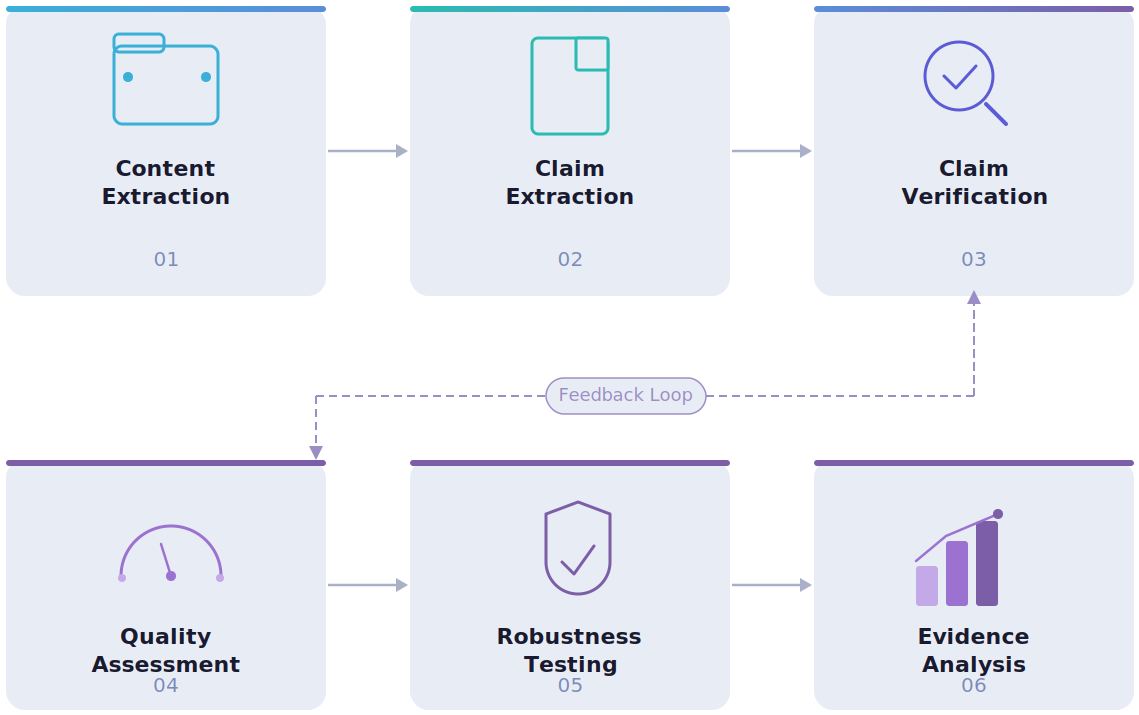
\includegraphics[width=\linewidth]{resources/venture_truth_architecture_light_larger_font.png}
    \caption{The \textsc{VentureTruth} pipeline architecture.}
    \label{fig:venture_truth_structure}
\end{figure}

As illustrated in Figure~\ref{fig:venture_truth_structure}, \textsc{VentureTruth} comprises six modules: \textit{Content Extraction}, \textit{Claim Extraction}, \textit{Claim Verification}, \textit{Quality Assessment}, \textit{Robustness Testing}, and \textit{Evidence Analysis}. Below, we summarize the purpose of each component.
\\
\\
\textbf{Content Extraction.} This module ingests raw materials (e.g., PDFs) and structured metadata (e.g., CSVs) and produces a unified representation. It combines standard PDF parsing with OCR to support both digitally encoded and scanned, image-heavy documents.
\\
\\
\textbf{Claim Extraction.} This module identifies atomic, external-facing factual claims while filtering out subjective or promotional statements. Compound claims are decomposed to ensure one-to-one correspondence between claims and verifiable propositions.
\\
\\
\textbf{Claim Verification.} For each claim, the verifier retrieves web evidence and outputs a verdict with confidence according to the predefined rules. Verification is embedded in an iterative refinement loop that incorporates feedback from the quality assessment component.
\\
\\
\textbf{Quality Assessment.} This module critiques verification outputs along three dimensions: reasoning soundness, source relevance/independence, and confidence calibration. It produces structured feedback (e.g., refining queries, resolving entity aliases, tightening evidence thresholds) that is injected into subsequent verification iterations.
\\
\\
\textbf{Robustness Testing.} This module re-verifies claims under prompt variations (neutral, evidence-focused, sceptical) and measures verdict agreement and confidence variance. Unstable claims are flagged for abstention or manual review.
\\
\\
\textbf{Evidence Analysis.} This module categorizes sources (news, regulatory, industry, official, social, other) and computes evidence diversity (e.g., unique domains per claim) to analyze how evidentiary breadth relates to model confidence. This is the last step of the pipeline that produces the final output. Sample output of the pipeline can be found in Appendix \ref{appendix:sample_output}.

\subsection{Implementation Details}
The \textsc{VentureTruth} pipeline is implemented in Python and parametrized via a single YAML configuration that specifies paths, model parameters, and operational thresholds.
\\
\\
\textbf{Content Extraction.} The ingestion phase aggregates metadata from \texttt{csv\_path} and documents from \texttt{pdf\_folder}. It uses \texttt{PyPDF2} for standard text extraction and \texttt{pdf2image} and \ texttt {pytesseract} for text extraction from images. The extracted data is matched against the metadata and stored as structured JSON, combining metadata and document text.
\\
\\
\textbf{Claim Extraction.} It uses an LLM to generate candidate claims with unique identifiers and a claim-confidence score. Prompts enforce atomicity, falsifiability, and external-facing relevance. To minimize model hallucination, we set the temperature to 0.
\\
\\
\textbf{Claim Verification.} Verification is managed by a \texttt{SearchManager} and \texttt{ClaimVerifier}.
\\
\\
The \texttt{SearchManager} queries the Perplexity API (\texttt{sonar-pro}) and performs:
\begin{enumerate}
    \item \textbf{Entity resolution:} identify the primary entity and aliases (e.g., legal vs.\ brand names);
    \item \textbf{Multi-angle querying:} target (a) official announcements, (b) independent journalism, and (c) regulatory/third-party registries;
    \item \textbf{Result triage:} label URLs by relevance (\texttt{HIGH, MEDIUM, LOW, OFF\_TOPIC}) and retain top results.
\end{enumerate}
~\\
The \texttt{ClaimVerifier} invokes an LLM at temperature 0 to output a structured verdict and confidence score, following calibration rules:
\begin{itemize}
    \item \texttt{INSUFFICIENT\_EVIDENCE}: triggered when evidence is absent, dependent/self-published, or inconclusive; confidence is bounded to a score range of $0.3$ -- $0.5$.
    \item \texttt{SUPPORTED}: requires independent corroboration; high confidence ($>0.8$) requires at least two robust independent sources.
    \item \textbf{Source independence:} entity websites and press releases are treated as dependent and are insufficient alone for high-confidence support.
\end{itemize}
~\\
\textbf{Quality Assessment.} The \texttt{QualityChecker} uses a LLM (temperature 0.1) to critique preliminary reports and assigns continuous scores in $[0,1]$ for Reasoning Quality, Source Relevance/Independence, and Certainty Calibration. Scores are discretized into \texttt{EXCELLENT}, \texttt{GOOD}, \texttt{ACCEPTABLE}, \texttt{POOR}, or \texttt{CRITICAL}. If ratings fall below the threshold, the system generates targeted recommendations that guide a subsequent verification iteration.
\\
\\
\textbf{Robustness Testing.} The \texttt{RobustnessChecker} re-verifies claims across neutral, evidence-focused, and sceptical prompts and tracks verdict agreement and confidence variance. Claims with agreement below a threshold of $<0.67$ or high variance are flagged as unstable, triggering forced abstention or manual review.
\\
\\
\textbf{Evidence Analysis.} The \texttt{ClaimsEvidence\allowbreak Analyzer} assigns sources to \texttt{News}, \texttt{Regulatory}, \texttt{Industry}, \texttt{Official}, \texttt{Social}, and \texttt{Other} via URL/domain heuristics and computes descriptive statistics (e.g., number of sources and unique domains per claim) to analyze the relationship between evidentiary diversity and confidence.